
\documentclass[11pt]{article}
\usepackage[margin=0.85in]{geometry}
\usepackage{graphicx}
\usepackage{booktabs}
\usepackage{float}
\usepackage{hyperref}
\usepackage{amsmath}
\usepackage{amssymb}
\usepackage{array}
\usepackage{caption}
\usepackage{microtype}

\title{FTS-Diffusion Replication Attempt: Results and Diagnostic Report}
\author{}
\date{May 11, 2026}

\begin{document}
\maketitle

\section{What We Did}

\begin{itemize}
\item Collected the paper-consistent artifacts: 7 TATR matrices, 7 final figures under \texttt{figures/}, reference TMTR/TATR summaries, SISC outputs, and bundled reference figures.
\item Aggregated each TATR matrix over 30 runs and plotted mean MAE with one-standard-deviation bands.
\item Added the predictable-drift component as a separate diagnostic, but did not report FTS-Diffusion drift numbers because no ordered generated sample paths are present in this checkout.
\end{itemize}

\section{Available Artifacts}

The report uses the paper-consistent K choices: GOOG K=11, ZCF K=11, and SP500 K=14. Other local artifacts, such as ZCF K=14, are excluded from the tables and figures for consistency. The TATR matrices have columns 0, 10, \ldots, 100, interpreted as synthetic augmentation percentages. The full file list and plot list are stored in \texttt{manifest.json} and \texttt{tables/tatr\_summary.csv}. No real generated-sample drift diagnostic outputs are present in this checkout; this report therefore does not claim no-drift results for FTS-Diffusion samples.

\section{TATR Matrix Results}

Table~\ref{tab:tatr-summary} summarizes the pulled TATR matrices. Negative change means lower MAE than the 0\% synthetic baseline.

\begin{table}[H]
\centering
\small
\caption{Summary of pulled TATR result matrices. Negative change means lower MAE than the 0\% synthetic baseline.}
\label{tab:tatr-summary}
\resizebox{\linewidth}{!}{%
\begin{tabular}{lrrrrrrrrr}
\toprule
Data & K & Variant & Runs & 0\% mean & Best \% & Best mean & Best change \% & 100\% mean & 100\% change \% \\
\midrule
GOOG & K11 & authors & 30 & 0.0119 & 0 & 0.0119 & 0.0000 & 0.1308 & 1003.0943 \\
GOOG & K11 & single & 30 & 0.0119 & 0 & 0.0119 & 0.0000 & 0.0244 & 105.6372 \\
SP500 & K14 & authors & 30 & 0.0611 & 0 & 0.0611 & 0.0000 & 0.1886 & 208.3886 \\
SP500 & K14 & random\_init & 30 & 0.0611 & 0 & 0.0611 & 0.0000 & 0.1028 & 68.1659 \\
SP500 & K14 & single & 30 & 0.0611 & 50 & 0.0132 & -78.4489 & 0.0173 & -71.6390 \\
ZCF & K11 & authors & 30 & 0.0113 & 0 & 0.0113 & 0.0000 & 0.0198 & 75.0735 \\
ZCF & K11 & single & 30 & 0.0113 & 0 & 0.0113 & 0.0000 & 0.0600 & 430.8901 \\
\bottomrule
\end{tabular}%
}
\end{table}

\section{Updated TATR/TMTR Result Figures}

These are the newest final result PDFs under the repository \texttt{figures} directory, filtered to GOOG K=11, ZCF K=11, and SP500 K=14.

\begin{figure}[H]
\centering

\includegraphics[width=0.90\linewidth]{../../figures/goog/k11/authors/final.pdf}
\caption{Pulled final result figure for GOOG K11 authors.}
\end{figure}
\begin{figure}[H]
\centering

\includegraphics[width=0.90\linewidth]{../../figures/goog/k11/single/final.pdf}
\caption{Pulled final result figure for GOOG K11 single.}
\end{figure}
\begin{figure}[H]
\centering

\includegraphics[width=0.90\linewidth]{../../figures/sp500/k14/authors/final.pdf}
\caption{Pulled final result figure for SP500 K14 authors.}
\end{figure}
\begin{figure}[H]
\centering

\includegraphics[width=0.90\linewidth]{../../figures/sp500/k14/random_init/final.pdf}
\caption{Pulled final result figure for SP500 K14 random\_init.}
\end{figure}
\begin{figure}[H]
\centering

\includegraphics[width=0.90\linewidth]{../../figures/sp500/k14/single/final.pdf}
\caption{Pulled final result figure for SP500 K14 single.}
\end{figure}
\begin{figure}[H]
\centering

\includegraphics[width=0.90\linewidth]{../../figures/zcf/k11/authors/final.pdf}
\caption{Pulled final result figure for ZCF K11 authors.}
\end{figure}
\begin{figure}[H]
\centering

\includegraphics[width=0.90\linewidth]{../../figures/zcf/k11/single/final.pdf}
\caption{Pulled final result figure for ZCF K11 single.}
\end{figure}

\section{Reference Summary CSVs}

Table~\ref{tab:reference-summary} reproduces the bundled reference TMTR/TATR summary rows.

\begin{table}[H]
\centering
\scriptsize
\caption{Reference summary CSV rows bundled with the original FTS-Diffusion repository.}
\label{tab:reference-summary}
\begin{tabular}{lrr}
\toprule
Exp. & Idx & Avg \\
\midrule
TATR & 0 & 0.1509 \\
TATR & 1 & 0.1254 \\
TATR & 2 & 0.2129 \\
TATR & 3 & 0.2305 \\
TATR & 4 & 0.2004 \\
TATR & 5 & 0.2234 \\
TATR & 6 & 0.2071 \\
TATR & 7 & 0.2710 \\
TATR & 8 & 0.3173 \\
TATR & 9 & 0.2781 \\
TATR & 10 & 0.3084 \\
TMTR & 0 & 0.2959 \\
TMTR & 1 & 0.3117 \\
TMTR & 2 & 0.3299 \\
TMTR & 3 & 0.4419 \\
TMTR & 4 & 0.4973 \\
\bottomrule
\end{tabular}%
\end{table}

\section{SISC Pattern-Recognition Artifacts and Plots}

The local reference artifacts contain 14 SISC centroids and 704 segmentation boundary rows for SP500 K=14.

\begin{figure}[H]
\centering
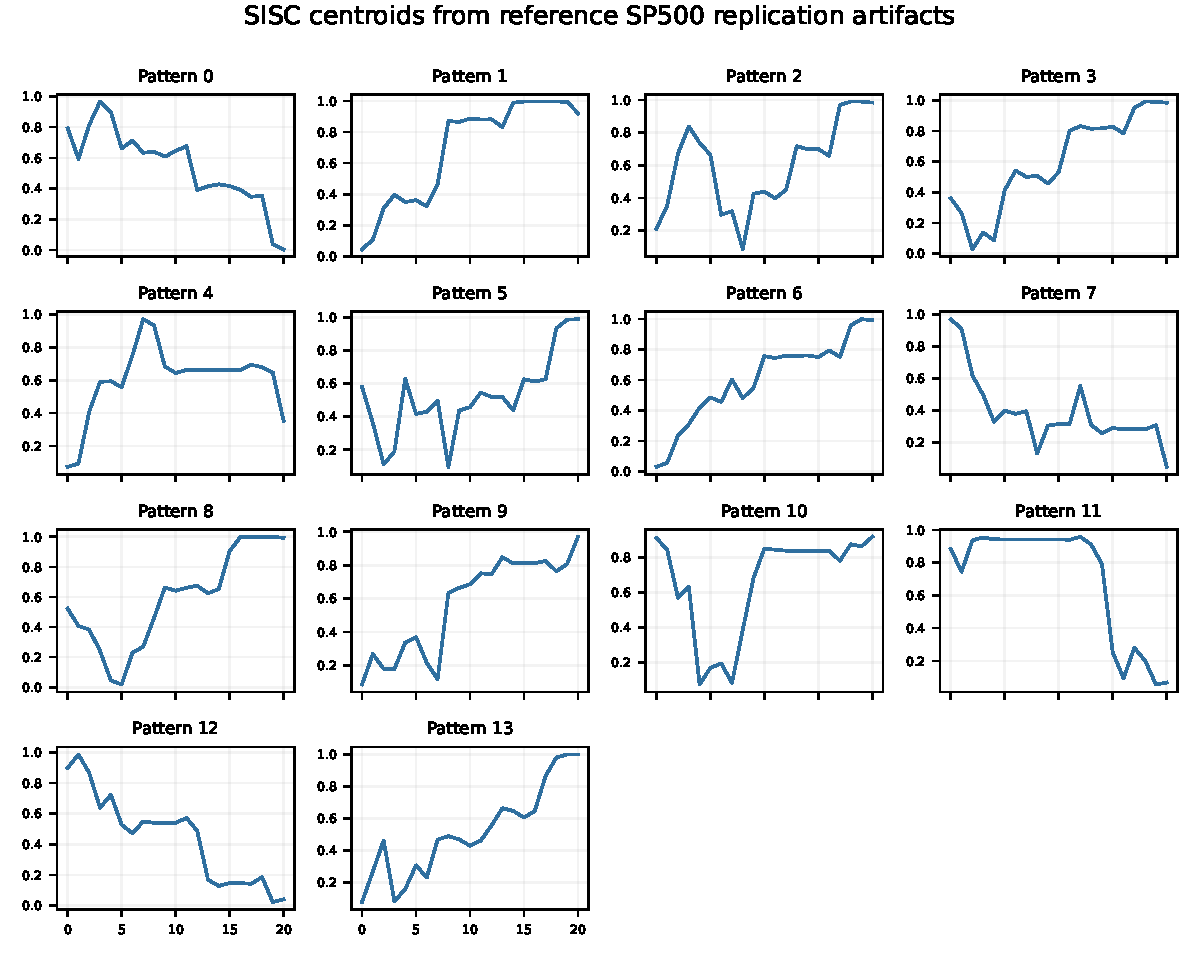
\includegraphics[width=0.90\linewidth]{figures/sisc_centroids.pdf}
\caption{SISC artifact plot: sisc centroids.}
\end{figure}
\begin{figure}[H]
\centering
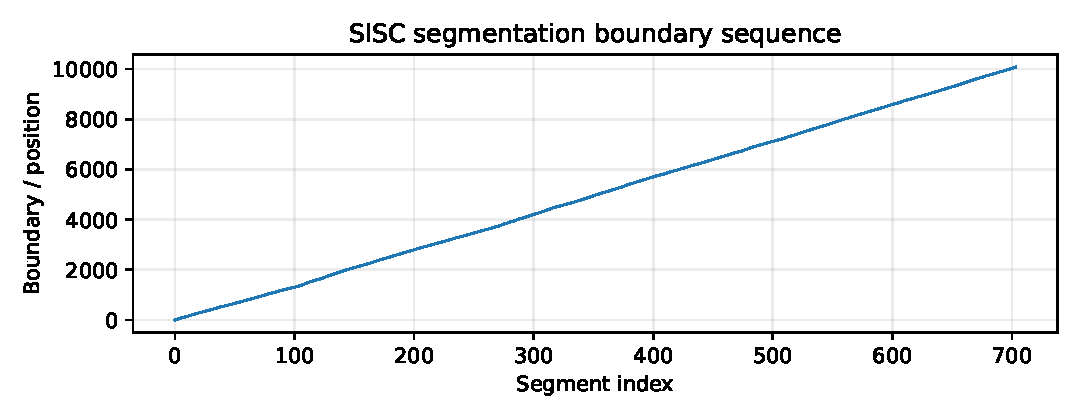
\includegraphics[width=0.90\linewidth]{figures/sisc_segmentation_boundaries.pdf}
\caption{SISC artifact plot: sisc segmentation boundaries.}
\end{figure}

\section{Bundled Stylized-Fact Figure}

\begin{figure}[H]
\centering

\includegraphics[width=0.92\linewidth]{../../fts-diffusion-ref/figs/stylized_fact.pdf}
\caption{Reference stylized-fact figure bundled with the FTS-Diffusion code.}
\label{fig:ref-stylized}
\end{figure}

\section{Predictable-Drift Extension Status}

The drift component targets the gap that matching stylized facts does not imply
\[
  \mathbb{E}[r_{t+1}\mid \mathcal{F}_t] = 0.
\]
It fixes
\[
  \omega_t = (1, r_t, r_{t-1}, |r_t|, |r_{t-1}|)
\]
and computes
\[
  \widehat{\delta} =
  \left\|
  \frac{1}{T}\sum_t r_{t+1}\omega_t
  \right\|_2.
\]
This is a finite-dimensional check, not a full no-arbitrage proof. Because no ordered generated return paths are present here, this PDF does not report drift statistics for actual FTS-Diffusion samples.

\section{Replication Caveats}

\begin{itemize}
\item The pulled \texttt{results/tatr/**/results\_matrix.csv} files are result matrices, not generated financial return paths.
\item The report does not include RCGAN, TimeGAN, or CSDI reruns.
\item The SISC artifacts and reference figures are bundled outputs from the reference directory; they support comparison, but are not proof that the full pipeline was freshly retrained in this checkout.
\item A full replication report should add training logs, generated sample CSVs, exact seeds, and final drift diagnostics once those outputs are available.
\end{itemize}

\end{document}
